% Cost-attribution ablation (DATA plot) — PLUM-128 verify, SHA-3 hasher, execute mode.
% Source: docs/precompile_soundness/uint256_mul_for_fp192.md (cumulative cycle counts).
% SP1:  289,778,709 -> 276,643,994 -> 240,857,140 -> 179,952,920  (-37.9%)
% RISC0: 812,646,400 -> ... -> 239,599,616  (-70.5%)
% Compile: pdflatex ablation_bars.tex
\documentclass[border=4pt]{standalone}
\usepackage{newtxtext,newtxmath}
\usepackage{pgfplots}
\pgfplotsset{compat=1.18}
\begin{document}
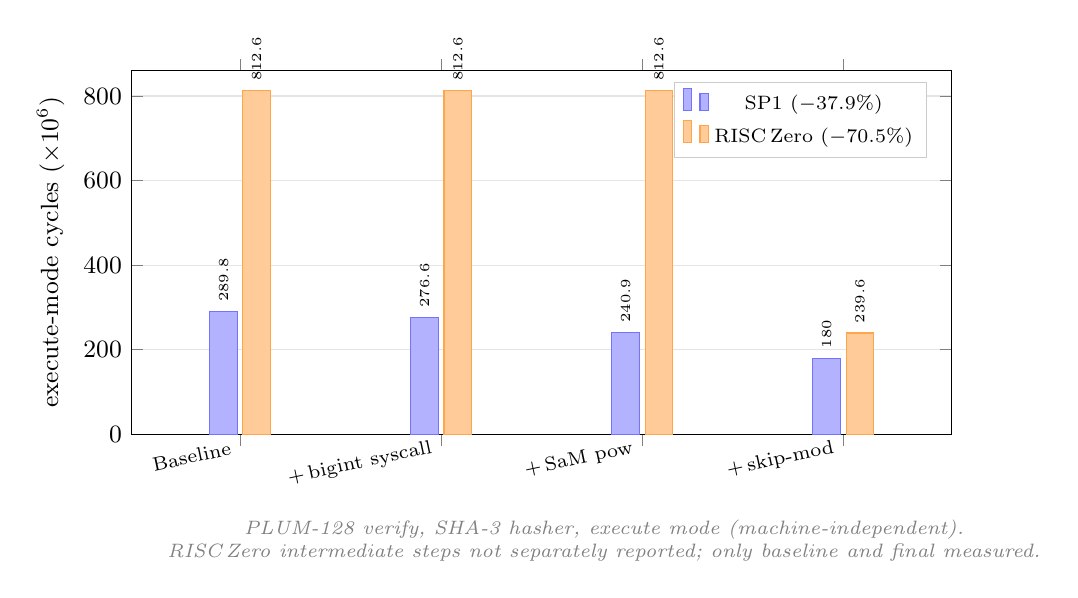
\begin{tikzpicture}
\begin{axis}[
  width=12cm, height=6.2cm,
  ybar, bar width=10pt,
  ymin=0, ymax=860,
  ylabel={execute-mode cycles ($\times 10^{6}$)},
  symbolic x coords={Baseline, {+\,bigint syscall}, {+\,SaM pow}, {+\,skip-mod}},
  xtick=data, x tick label style={font=\scriptsize,align=center,rotate=12,anchor=east},
  ymajorgrids, grid style={gray!20},
  legend style={at={(0.97,0.97)},anchor=north east,font=\scriptsize,draw=gray!40},
  nodes near coords, every node near coord/.append style={font=\tiny,rotate=90,anchor=west},
  enlarge x limits=0.18,
  font=\small,
]
% SP1 series (millions)
\addplot[fill=blue!30,draw=blue!55] coordinates
  {(Baseline,289.8) ({+\,bigint syscall},276.6) ({+\,SaM pow},240.9) ({+\,skip-mod},180.0)};
% RISC0 series (millions) -- only baseline + final measured in the doc
\addplot[fill=orange!40,draw=orange!70] coordinates
  {(Baseline,812.6) ({+\,bigint syscall},812.6) ({+\,SaM pow},812.6) ({+\,skip-mod},239.6)};
\legend{SP1 ($-37.9\%$), RISC\,Zero ($-70.5\%$)}
\end{axis}
\node[font=\scriptsize\itshape,gray,align=center] at (6cm,-1.35cm)
  {PLUM-128 verify, SHA-3 hasher, execute mode (machine-independent).\\
   RISC\,Zero intermediate steps not separately reported; only baseline and final measured.};
\end{tikzpicture}
\end{document}
